\documentclass[a4paper]{book}

%\usepackage[english, greek]{babel}
\usepackage{alphabeta} 
\usepackage{enumitem} 
\usepackage{mathtools}
\usepackage{amsmath, amssymb} 
\usepackage{amsthm}
\usepackage{cancel} 
\usepackage[margin=0.70in]{geometry} 
\geometry{left=2.3cm,right=2.3cm,top=2.4cm,bottom=2.4cm}	%the p1age geometry as defined, A4=210x297mm
\usepackage{graphicx}
\usepackage{wrapfig}
\usepackage[center]{caption}
\usepackage{textcomp}
\usepackage{tabto}
\usepackage{layout}
\usepackage{bm}
\usepackage{minipage-marginpar}
\usepackage[dvipsnames]{xcolor}
\usepackage{hyperref}
\usepackage{dutchcal}
\usepackage{derivative}
\usepackage{esint}
%\usepackage{biblatex}
\usepackage{subcaption}
\usepackage{caption}
\usepackage{fancyhdr}
\usepackage{booktabs}\usepackage{derivative}
\usepackage[flushleft]{threeparttable}
%\usepackage[capbesideposition=outside,capbesidesep=quad]{floatrow}
\usepackage{derivative}
\usepackage[thinc]{esdiff}
\usepackage{lipsum}
\usepackage{arydshln}
\usepackage{titlesec}
\usepackage{listings}
\usepackage{xcolor}
\usepackage{braket}
%%RENEW

\newtheorem{problem}{Άσκηση}
\newtheorem*{solution*}{Λύση}
\newtheorem{definition}{Ορισμός}[subsection]
\newtheorem{properties}{Ιδιότητες}[subsection]
\newtheorem{theorem}{Θεώρημα}[subsection]
\newtheorem{protash}{Πρόταση}[subsection]
\newtheorem{porisma}{Πόρισμα}[subsection]
\newtheorem{lemma}{Λήμμα}[subsection]
\newtheorem*{prooof}{Απόδειξη}
\newtheorem*{notes}{Παρατηρήσεις}
\newtheorem*{note}{Παρατήρηση}
\newtheorem*{app}{Εφαρμογή} 
\newtheorem*{example}{Παράδειγμα}
\newtheorem*{examples}{Παραδείγματα}


\newcommand\numberthis{\addtocounter{equation}{1}\tag{\theequation}}
%\renewcommand{\labelenumi}{\roman{enumi}}
\newcommand{\approxtext}[1]{\ensuremath{\stackrel{\text{#1}}{\approx}}}
\renewcommand{\figurename}{Εικόνα.}
\renewcommand{\tablename}{Πίνακας.}
%\renewcommand\refname{New References Header}
\renewcommand*\contentsname{Περιεχόμενα}
%\DeclareDerivative{\odv}{\mathrm{d}}


%Customize code block--------------------------------
\definecolor{codegreen}{rgb}{0,0.6,0}
\definecolor{codegray}{rgb}{0.5,0.5,0.5}
\definecolor{codepurple}{rgb}{0.58,0,0.82}
%\definecolor{backcolour}{rgb}{0.95,0.95,0.92}
\definecolor{backcolour}{rgb}{0.95, 0.95, 0.97}
\definecolor{crimsonglory}{rgb}{0.75, 0.0, 0.2}
\definecolor{darkcerulean}{rgb}{0.03, 0.27, 0.49}
\definecolor{indiagreen}{rgb}{0.07, 0.53, 0.03}

\lstdefinestyle{mystyle}{
    backgroundcolor=\color{backcolour},   
   % commentstyle=\color{codegreen},
    commentstyle=\color{indiagreen},
   % keywordstyle=\color{magenta},
   	keywordstyle=\color{crimsonglory},
    numberstyle=\tiny\color{codegray},
   % stringstyle=\color{codepurple},
   	stringstyle=\color{darkcerulean},
    basicstyle=\ttfamily\footnotesize,
    breakatwhitespace=false,         
    breaklines=true,                 
    captionpos=b,                    
    keepspaces=true,                 
    numbers=left,                    
    numbersep=5pt,                  
    showspaces=false,                
    showstringspaces=false,
    showtabs=false,                  
    tabsize=2
}
\lstset{style=mystyle}
%----------------------------------------------------




\title{Η μέθοδος Monte Carlo ή μέθοδος των τυχαίων αριθμών}
\author{Θωμόπουλος Σπυρίδων, ge19042}

\titleformat{\chapter}[hang]{\normalfont\huge\bfseries\color{black}}{\thechapter}{1cm}{}{}
%
\pagestyle{fancy}
\fancyhead{}
\fancyfoot{}
\fancyhead[LO,LE]{\textbf{04 Monte Carlo}}
\fancyfoot[CE,CO]{\thepage}







\begin{document}
%\selectlanguage{english}
\begin{titlepage}




\newcommand{\HRule}{\rule{\linewidth}{0.5mm}}

\includegraphics[width=8cm]{logo1.png}\\[1cm] 
\center 
\quad\\[1.5cm]
\textsl{\Large Εθνικό Μετσόβιο Πολυτεχνείο}\\[0.5cm] 
\textsl{\large Σχολή Εφαρμοσμένων Μαθηματικών και Φυσικών Επιστημών}\\[0.5cm] 
\makeatletter
\HRule \\[0.4cm]
{ \huge \bfseries \@title}\\[0.4cm] 
\HRule \\[1.5cm]
\begin{minipage}{0.4\textwidth}
\begin{flushleft} \large
\emph{Author:}\\
\@author 
\end{flushleft}
\end{minipage}
~
\begin{minipage}{0.4\textwidth}
\begin{flushright} \large

\end{flushright}
\end{minipage}\\[3cm]
\makeatother
%{\large An Assignment submitted for the UoS:}\\[0.5cm]
{\large \emph{Εργαστήριο Πυρηνικής Φυσικής \& Στοιχειωδών Σωματιδίων}}\\[0.5cm]
{\large \today}\\[2cm] 
\vfill 



\end{titlepage}

\begin{enumerate}
	\item[\textbf{Ερώτημα 1.}] 
	
	\begin{itemize}
		\item  \textbf{Ομοιόμορφη Κατανομή} 
			
				Αρχικά θα δούμε το πως αλλάζει η ομοιόμορφη κατανομή, που προέρχεται από την "γεννήτρια τυχαίων αριθμών" %$\frac{n_{i+1}}{m} = \alpha \frac{n_i}{m} mod(m)$
				\begin{equation}\label{eq1}
				n_{i+1}=\alpha n_imod(m)
				\end{equation}
				 για seed $n_0 = 13$, καθώς μεταβάλλεται ο αριθμός των "τυχαίων αριθμών" που επιλέγουμε (δηλαδή το μέγιστο i της ακολουθίας) και ο αριθμός των bins (δηλαδή το εύρος των διαστημάτων σε ένα ιστόγραμμα).
				
				Θέλουμε να δούμε το πως αλλάζει η κατανομή τυχαίων αριθμών που προέρχονται από μία κανονική κατανομή
				
				Χρησιμοποιώντας το πρόγραμμα "example1.m" σταθεροποιούμε τον αριθμό των $bins=10$ και μεταβάλλουμε τον αριθμό των τυχαίων αριθμών $Nrand=\{50, 100, 1000, 10000, 100000\}$. Τα αποτελέσματα φαίνονται στις Εικόνες (\ref{fig1}a-e)
\begin{figure}[h!]
    \centering
    \subfloat[\centering Nrand=50]{{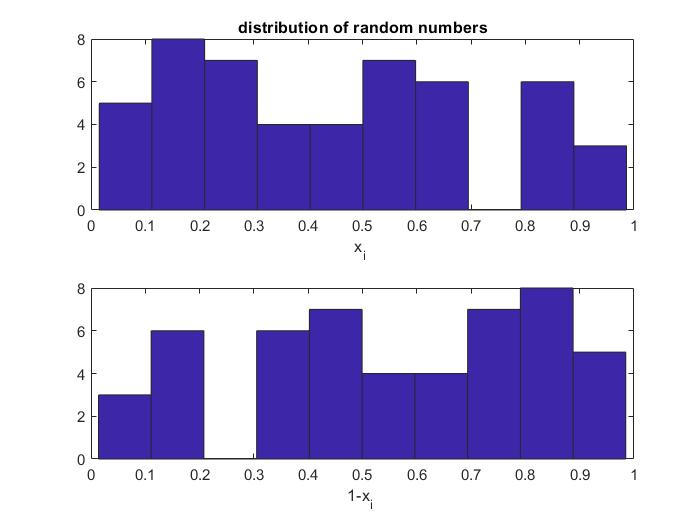
\includegraphics[width=6cm]{Q1/H_N50_b10.jpg} }}%
    \qquad
    \subfloat[\centering Nrand=100]{{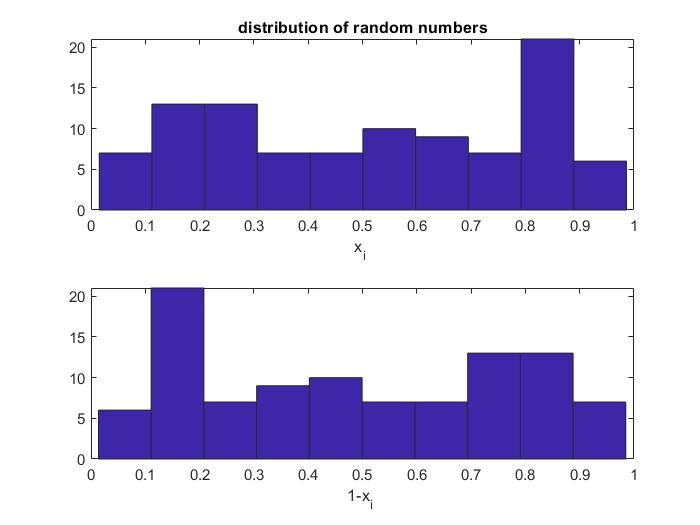
\includegraphics[width=6cm]{Q1/H_N100_b10.jpg} }}%
    \qquad
    \subfloat[\centering Nrand=1000]{{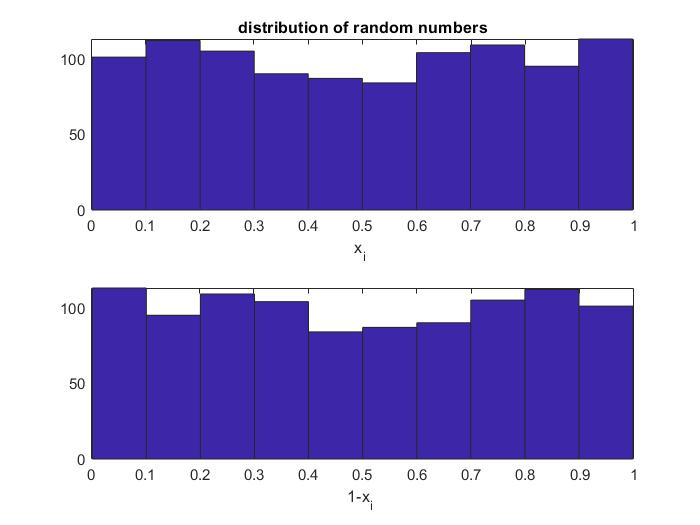
\includegraphics[width=6cm]{Q1/H_N1000_b10.jpg} }}%
    \qquad
    \subfloat[\centering Nrand=10000]{{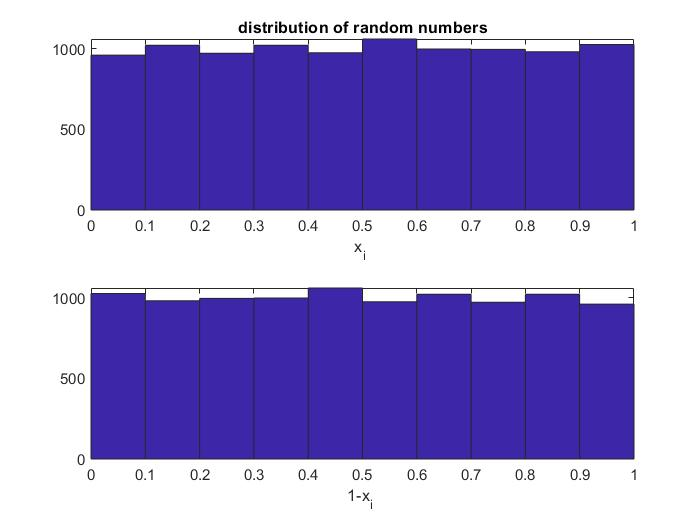
\includegraphics[width=6cm]{Q1/H_N10000_b10.jpg} }}%
    \qquad
    \subfloat[\centering Nrand=100000]{{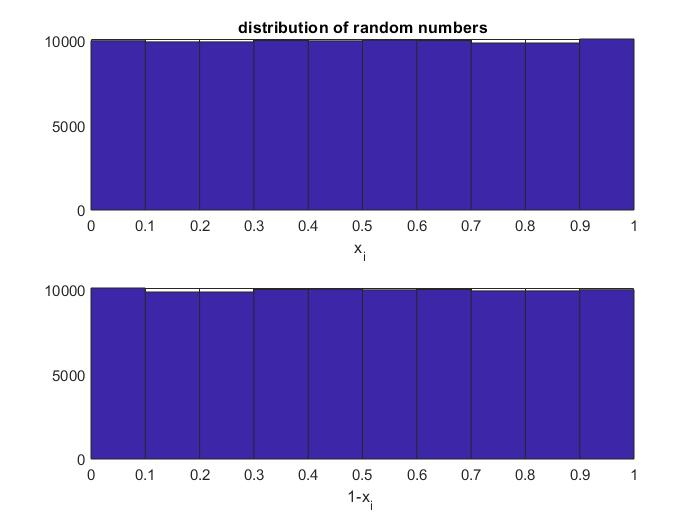
\includegraphics[width=6cm]{Q1/H_N100000_b10.jpg} }}%
    \caption{bins=10}%
    \label{fig1}%
\end{figure}				
			Ομοίως, σταθεροποιούμε τον αρθιθμό των $bins=100$ και μεταβάλλουμε τον αριθμό των τυχαίων αριθμών $Nrand=\{50, 100, 1000, 10000, 100000, 100000\}$. Τα αποτελέσματα φαίνονται στις Εικόνες (\ref{fig2}a-f)	
				
	\begin{figure}[h!]
    \centering
    \subfloat[\centering Nrand=50]{{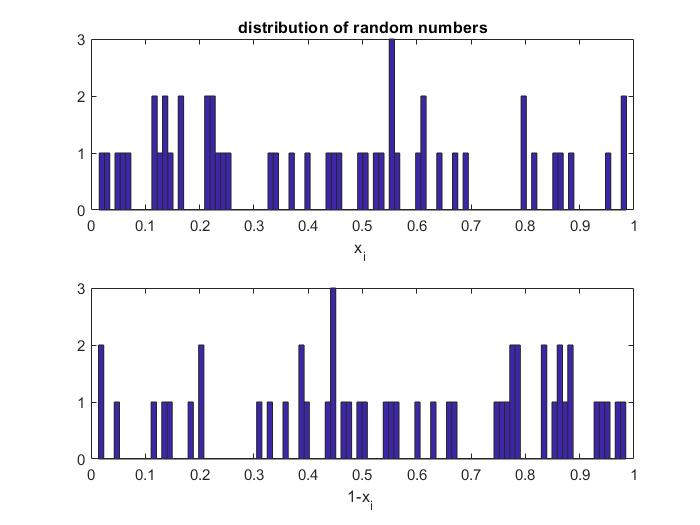
\includegraphics[width=6cm]{Q1/H_N50_b100.jpg} }}%
    \qquad
    \subfloat[\centering Nrand=100]{{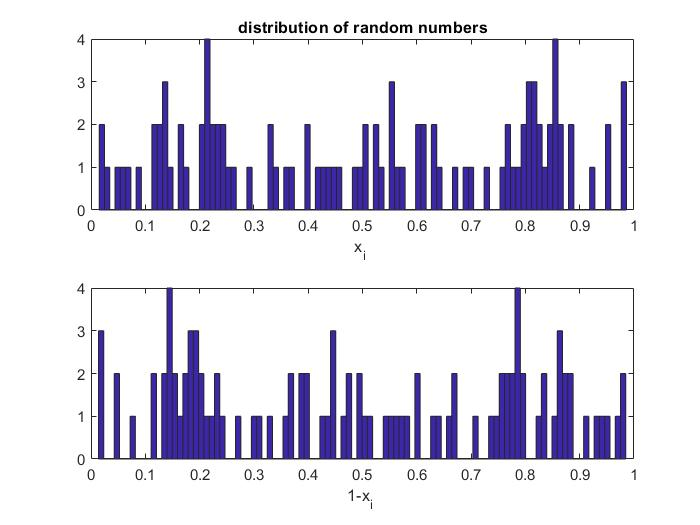
\includegraphics[width=6cm]{Q1/H_N100_b100.jpg} }}%
    \qquad
    \subfloat[\centering Nrand=1000]{{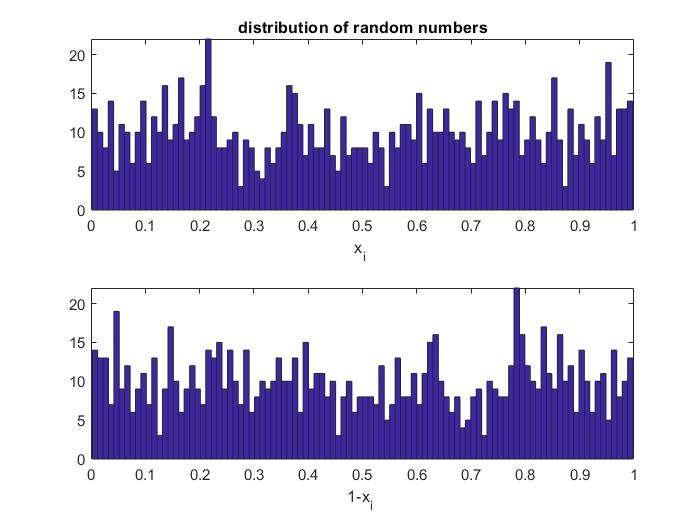
\includegraphics[width=6cm]{Q1/H_N1000_b100.jpg} }}%
    \qquad
    \subfloat[\centering Nrand=10000]{{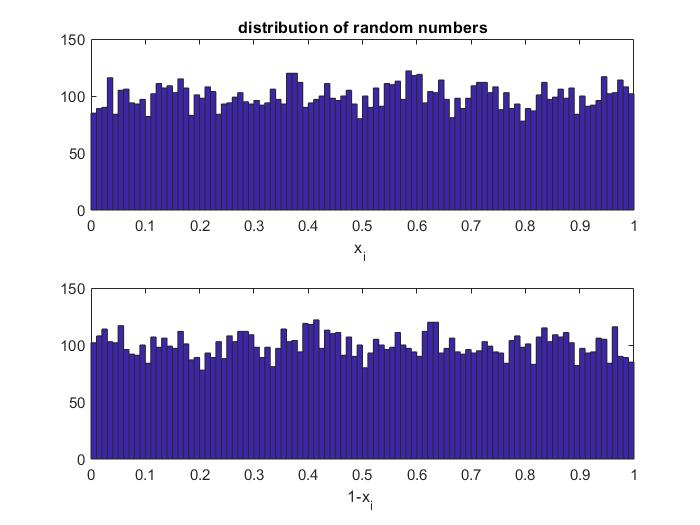
\includegraphics[width=6cm]{Q1/H_N10000_b100.jpg} }}%
    \qquad
    \subfloat[\centering Nrand=100000]{{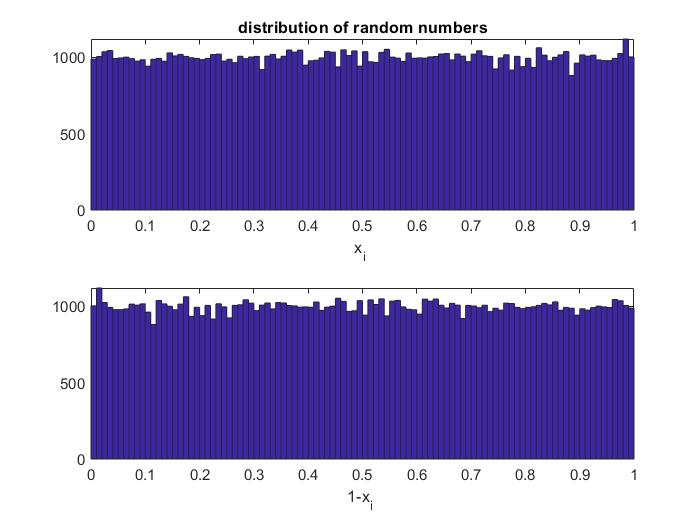
\includegraphics[width=6cm]{Q1/H_N100000_b100.jpg} }}%
    \qquad
    \subfloat[\centering Nrand=100000]{{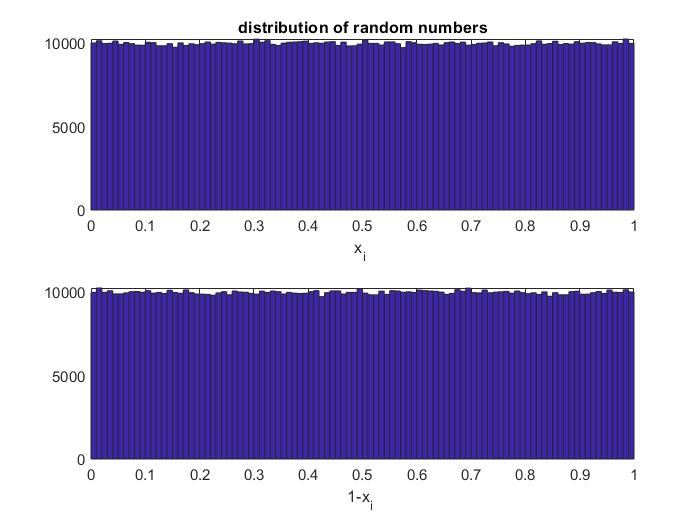
\includegraphics[width=6cm]{Q1/H_N1000000_b100.jpg} }}%
    \caption{bins=100}%
    \label{fig2}%
\end{figure}				
				
			Στις δύο περιπτώσεις για $bins=10, 100$ παρατηρούμε πως όταν το πλήθος των τυχαίων αριθμών αυξάνεται τότε η κατανομή τους συγκλίνει προς την ομοιόμορφη. Στην πρώτη περίπτωση αυτό φαίνεται από $Nrand=1000$ ενώ στην δεύτερη από $Nrand=10000$. Συνεπώς, μπορούμε να συμπεράνουμε πως όσο αυξάνουμε το binning χρειαζόμαστε όλο και μεγαλύτερο πλήθος τυχαίων αριθμών προκειμένου να προσεγγίσουμε την ομοιόμορφη κατανομή. Ο μετασχηματισμός $x_i\rightarrow 1-x_i$ συμπεριφέρεται όπως και το $x_i$.
		\item \textbf{Gaussian Κατανομή}
		 	Τώρα θέλουμε να κάνουμε το ίδιο με πριν, μόνο που οι τυχαίοι αριθμοί θα προέρχονται από μία Gaussian κατανομή. Επιλέγουμε seed, $n_0=13$ και επαναλαμβάνουμε τα ίδια βήματα με πριν χρησιμοποιώντας τώρα το αρχείο "example2.m". 
		 	Τα αποτελέσματα φαίνονται στις Εικόνες (\ref{fig3}a-e) για $bins=10$ και στις Εικόνες (\ref{fig4}a-e) για $bins=100$
		 	
	\begin{figure}[h!]
    \centering
    \subfloat[\centering Nrand=50]{{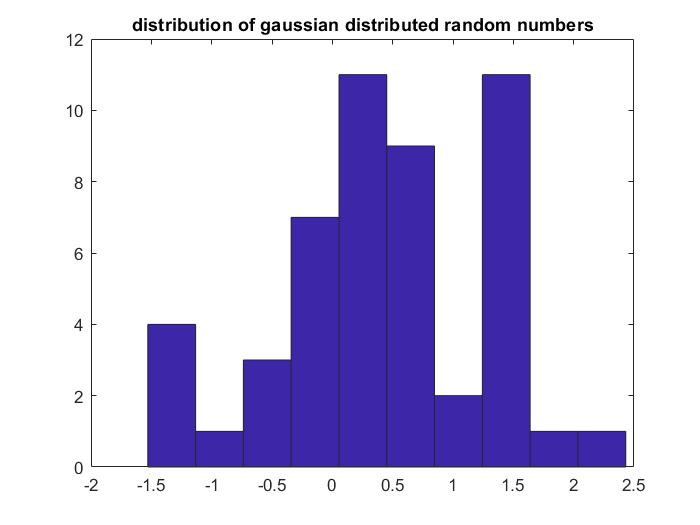
\includegraphics[width=5cm]{Q1/G_N50_b10.jpg} }}%
    \qquad
    \subfloat[\centering Nrand=100]{{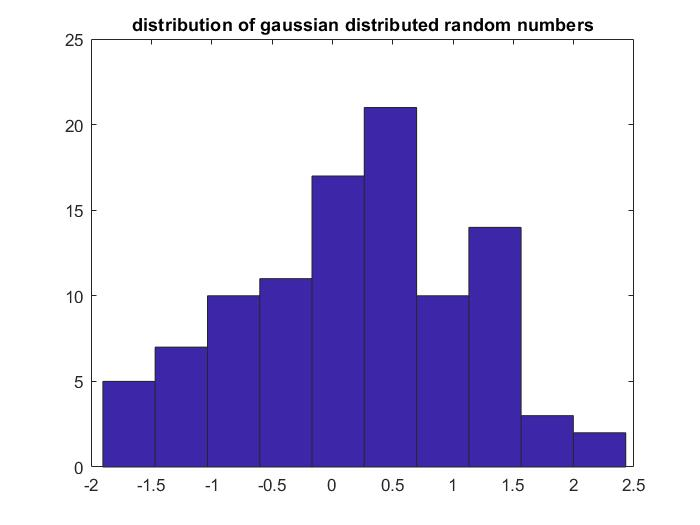
\includegraphics[width=5cm]{Q1/G_N100_b10.jpg} }}%
    \qquad
    \subfloat[\centering Nrand=1000]{{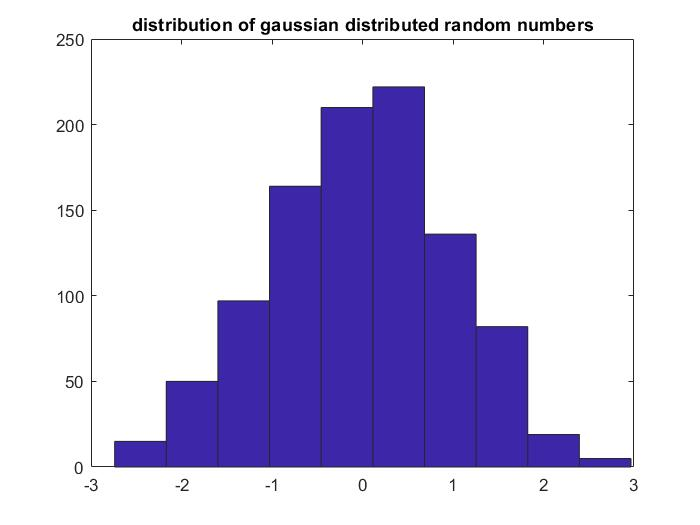
\includegraphics[width=5cm]{Q1/G_N1000_b10.jpg} }}%
    \qquad
    \subfloat[\centering Nrand=10000]{{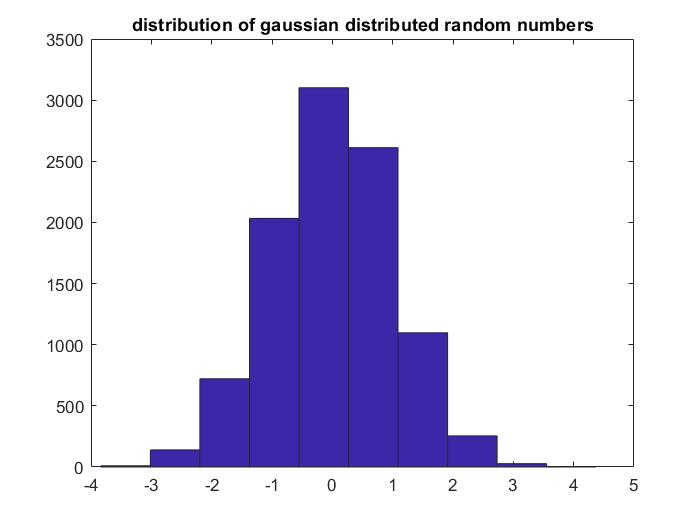
\includegraphics[width=5cm]{Q1/G_N10000_b10.jpg} }}%
    \qquad
    \subfloat[\centering Nrand=100000]{{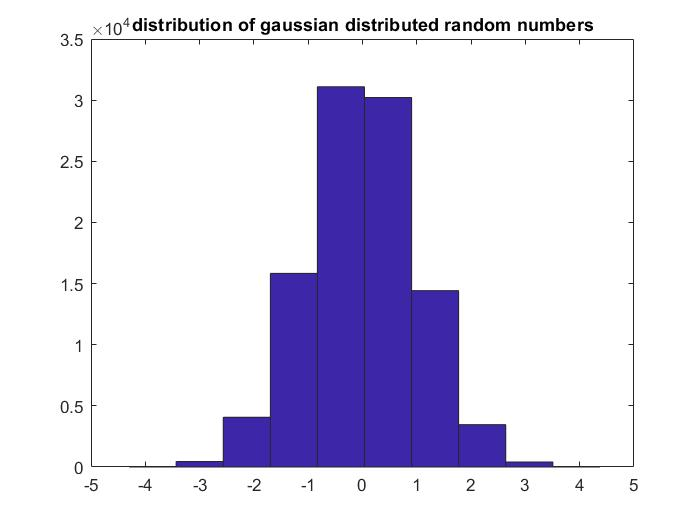
\includegraphics[width=5cm]{Q1/G_N100000_b10.jpg} }}%
    \caption{bins=10}%
    \label{fig3}%
\end{figure}		 	
		 	
	\begin{figure}[h!]
    \centering
    \subfloat[\centering Nrand=50]{{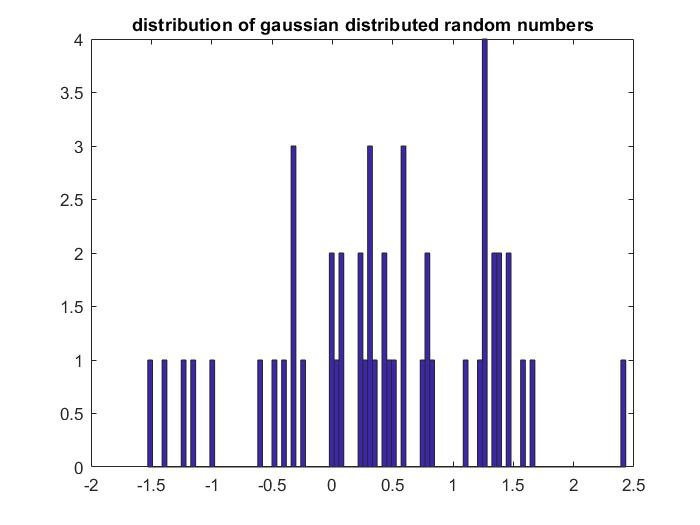
\includegraphics[width=6cm]{Q1/G_N50_b100.jpg} }}%
    \qquad
    \subfloat[\centering Nrand=100]{{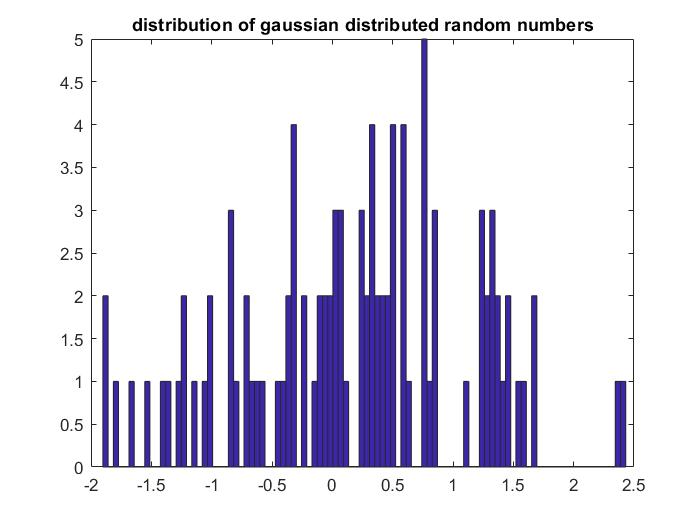
\includegraphics[width=6cm]{Q1/G_N100_b100.jpg} }}%
    \qquad
    \subfloat[\centering Nrand=1000]{{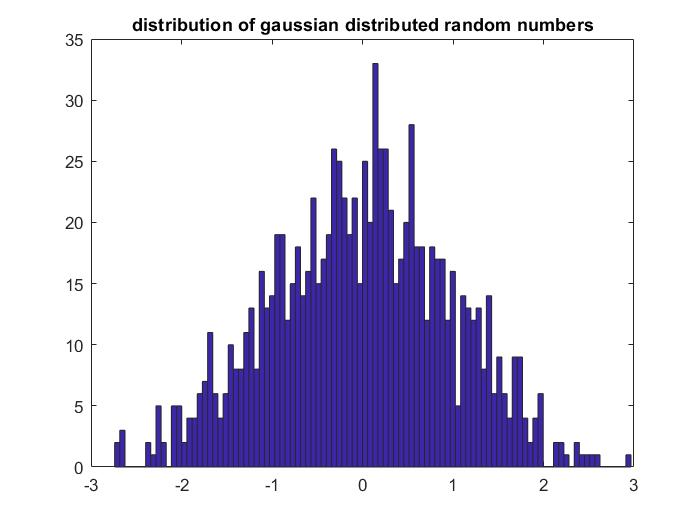
\includegraphics[width=6cm]{Q1/G_N1000_b100.jpg} }}%
    \qquad
    \subfloat[\centering Nrand=10000]{{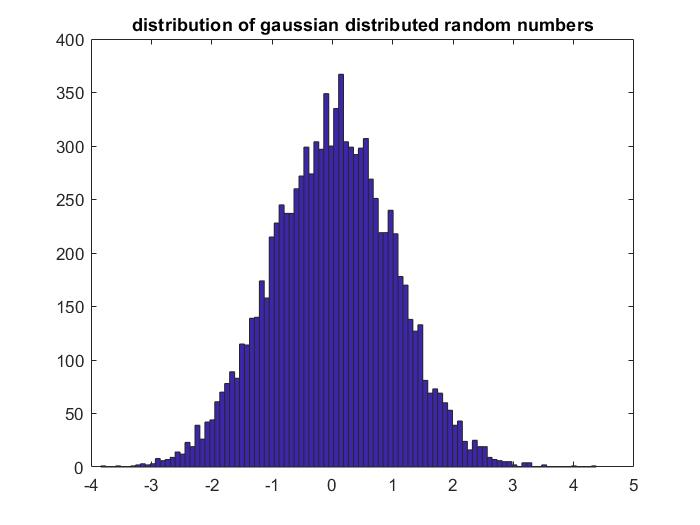
\includegraphics[width=6cm]{Q1/G_N10000_b100.jpg} }}%
    \qquad
    \subfloat[\centering Nrand=100000]{{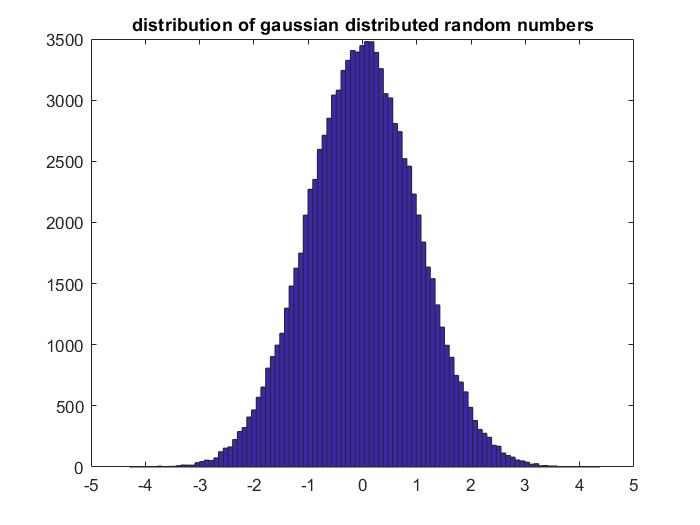
\includegraphics[width=6cm]{Q1/G_N100000_b100.jpg} }}%
    \caption{bins=100}%
    \label{fig4}%
\end{figure}
		 	
		 	
		 	Ομοίως με πριν, παρατηρούμε πως στις δύο περιπτώσεις $bins=10,100$ η κατανομή αρχίζει να γίνεται ξεκάθαρη από διαφορετικά πλήθη τυχαίων αριθμών, $Nrand=1000$ στην πρώτη περίπτωση και $Nrand=10000$ στην δεύτερη. Άρα πάλι μπορούμε να συμπεράνουμε πως αυξάνοντας το binning  αυξάνεται και το πλήθος τυχαίων αριθμών που απαιτούνται για να πάρουμε την Gaussian κατανομή.
	\end{itemize}	 
	
	
	%%%%%%%%%%%%%%%%%%%%%%%%%%%%%%%%%%%%%%%%%%%%%%%%%    2ND QUESTION %%%%%%%%%%%%%%%%%%%%%%%%%%%%%%%%%%%%%%%%%%%%%%%%%%%%%%%%%%%%%%%%%%%%%%
	\item[\textbf{Ερώτημα 2.}]	
		Τώρα. χρησιμοποιώντας το πρόγραμμα $pi1.m$ θα υπολογίσουμε την τιμή του $\pi/4$. Αρχικά, παράγουμε δύο ακολουθίες από ομοιόμορφα κατανεμημένα τυχαίους αριθμούς $(x_{i1},x_{i2})$ με βάση την σχέση (\ref{eq1}) οι οποίες θα έχουν διαφορετικά seeds, $seed_1 = 11$, $seed_2 = 7$. Άρα θα έχουμε Nrad ζευγάρια τυχαίων αριθμών εντός ενός τετραγώνου πλευράς 1. Εντός αυτού του τετραγώνου υπάρχει το ένα τεταρτοκύκλιο του μοναδιαίου κύκλου το οποίο έχει εμβαδό $\pi/4$. Άρα περιμένουμε πως ο λόγος $N_{in}/N_{total}$, του πλήθους των ζευγαριών που πέφτουν εντός του τεταρτοκυκλίου (δηλδή που έχουν $x_{i1}^2+x_{i2}^2<1$) προς το συνολικό πλήθος των ζευγαριών θα τείνει στο $\pi/4$ όταν πάρουμε μεγάλο αριθμό σημείων: 
			\begin{align}\label{2}
				       \braket{\pi/4} =& \frac{N_{in}}{N_{total}}\\ \vspace{-1cm}
			     \delta(\pi/4) =& \frac{1}{N_{total}}\sqrt{\frac{N_{in}(N_{total}-N_{in})}{N_{total}-1}}
			\end{align}
		Τρέχουμε το πρόγραμμα για διάφορες τιμές του Nrand. Τα αποτελέσματα φαίνονται στον παρακάτω Πίνακα (\ref{mat1}) 
		\begin{table}[h!]
			\centering
			\begin{tabular}{r|r|r|r|r}
				$seed_1$ & $seed_2$ &   Nrand   & $\braket{\pi/4}$ & $\delta(\pi/4)$ \\ \hline \hline	
				11       &    7     &      $10^1$   &    0.80000   & 0.07746 \\
				11       &    7     &     $10^2$   &    0.740000  & 0.04271 \\
				11       &    7     &    $10^3$   &    0.786000  & 0.01293 \\
				11       &    7     &   $10^4$   &    0.787000  & 0.00409 \\
				11       &    7     &  $10^5$   &    0.785510  & 0.00130 \\	
				11       &    7     & $10^6$   &	 0.784228  & 0.00041 \\
				11       &    7     &$10^7$   &    0.784447  & 0.00013
		\end{tabular}
			\caption{Τιμές του π/4 για διάφορα πλήθη Nrand τυχαίων ζευγραριών }
			\label{mat1}
		\end{table}
		
	Δεδομένου ότι η πραγματική τιμή είναι $\pi/4=0.785398 $, παρατηρούμε πως πράγματι για αυξανόμενο αριθμό σημείων ο λόγος τείνει στο $\pi/4$ και το σφάλμα γίνεται όλο και μικρότερο.
	
	Η παραπάνω μέθοδος έχει το πλεονέκτημα ότι είναι πολύ απλή στην κατανόηση και την υλοποίησή της και γρήγορη για μικρές τιμές του Nrand. Ωστόσο, παρ'ολο που φαίνεται να συγκλίνει στο π/4 η σύγκλιση θα είναι τόσο αργή ώστε όταν αυξήσουμε περεταίρω το πλήθος των τυχαίων αριθμών που παίρνουμε θα φτάσουμε τον υπολογιστή στα όριά του. Άρα, αν θέλουμε μία πρόχειρη εκτίμηση του π/4 θα μπορούσαμε να πούμε ότι είναι σχετικά καλή ενώ αν θέλαμε να υπολογίσουμε με ακρίβεια πολλά σημαντικά σημεία του η μέθοδος δεν είναι και τόσο αξιόπιστη. Η γραφική παράσταση $Nrand-\pi/4$ φαίνεται στην Εικόνα (\ref{fig5})
	
	\begin{figure}[h!]
		\centering
		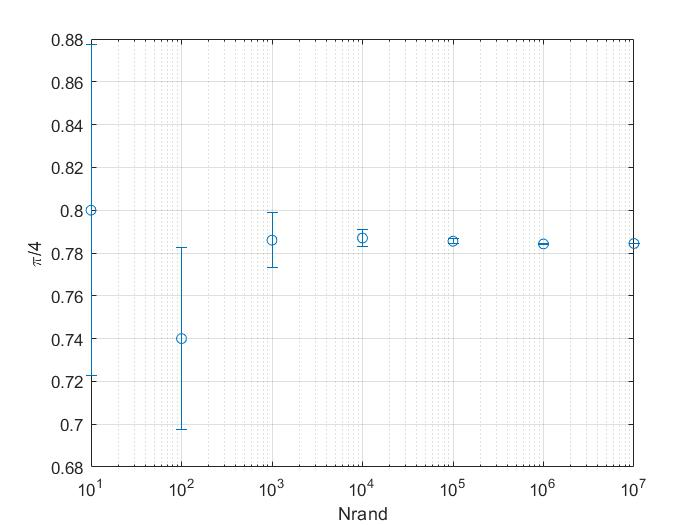
\includegraphics[scale=0.4]{Q2/nrand-pi4.jpg}
		\caption{Γραφική παράσταση Nrand-$\pi/4$ με λογαριθμικό άξονα x}
		\label{fig5}
	\end{figure}
	
	
	
	%%%%%%%%%%%%%%%%%%%%%%%%%%%%%%%%%%%%%%%%%%%%%% QUEST 3 %%%%%%%%%%%%%%%%%%%%%%%%%%%%%%%%%%%%%%%%%%%%%%%%%%%%%%%
	\item[\textbf{Ερώτημα 3.}]	
		Τώρα θα χρησιμοποιήσουμε την παραπάνω μέθοδο για να προσομοιώσουμε τον νόμο των ραδιενεργών διασπάσεων 
		\begin{align}\label{eq4}
			N = N_0 e^{-t/\tau}
		\end{align}
		


		όπου Ν ο αριθμός αδιάσπαστων πυρήνων, $N_0$ ο αρχικός αριθμός πυρήνων, t ο χρόνος και $\tau$ ο μέσος χρόνος ζωής του πυρνήνα που μελετάμε. Συγκεκριμένα θα ξεκινήσουμε με $seed=17$ και με $N_0=10^3$ ενώ θα μεταβάλλουμε το πλήθος των τυχαίων αριθμών που παίρνουμε από $Nrand=\{50, 10^3, 10^6\}$. Επίσης, θα πάρουμε τελικό χρόνο $t_f = 2700sec$ και κάθε $\Delta t = 100 sec$ θα αποθηκεύουμε τον αριθμό αδιάσπαστων πυρήνων που έχουν απομείνει στο σύστημά μας, σαν να επρόκειτο για πειραματικές μετρήσεις, ώστε εν τέλει να κάνουμε μία γραφική παράσταση $t-N(t)$. Οι μικροαλλαγές στον κώδικα φαίνονται παρακάτω (τις έχω σημειώσει με ****) και επίσης στο αρχείο "radiodec2\_Q3\_modified.m" και στον 	Πίνακα (\ref{mat2}) φαίνονται οι τιμές των πυρήνων συναρτήσει του χρόνου για τα  $Nrand = \{50, 10^3, 10^6\}$. Ακόμη, στον Πίνακα (\ref{mat3}) φαίνονται οι τιμές της παραμέτρου $-1/\tau$ με τα σφάλματά τους και επίσης το τ.
		
	
	\begin{lstlisting}[language=Matlab]
% neutron decay part2

N0=input        ('Number of neutrons at t=0                : ');
Iseed = input   ('Random number seed                       : ');
end_time = input('Enter time t                             : ');
Nrand = input   ('Number of random numbers to be generated : ');

%Nrand = N0;
rand('seed',Iseed);
Irand = rand(1,Nrand);

Nund = 0;
Nd = 0;
tend = end_time;
Probt = 1 - exp(-(tend/886.7));  % prob  decay
disp('---------------------------------')
disp('----#of undec nuceus 0:100:tend----')
disp('---------------------------------')
Nucl_undec = [];                            %****** contains the tnumber of undecayed at every 100sec
for t = 0:100:tend   % ************** loop that runs over all t from 0 to tend
    Nund = 0; Nd = 0;
    prob = 1 - exp(-(t/886.7));   % prob  decay
    
    for k = 1:Nrand
     if prob <= Irand(k)
       Nund = Nund + 1;
     else
     Nd = Nd + 1;
     end
    end
    i  = round(t/100);                          % ****
    Nucl_undec(i+1) = round(Nund*N0/Nrand);	    % ****array which contains the undec. nucl. for every Dt=100 from 0 to tend      
    fprintf('%i ', round(Nund*N0/Nrand));
end
Nundec = round(Nund*N0/Nrand);

fprintf('\n---------------------------\nNumber of undecayed neutrons after %i seconds: %i \n',end_time,Nundec);
tt = 0:100:2700;
%% FITTING SECTION
[xData, yData]   = prepareCurveData( tt, Nucl_undec );
ft               = fittype('exp1');
opts             = fitoptions( 'Method', 'NonlinearLeastSquares' );
%opts.Display     = 'off';
opts.StartPoint = [1000.0 0.0];
[fitresult, gof] = fit( xData, yData, ft, opts );
fitresult

figure( 'Name', 't - N(t)' );
h1 = plot( fitresult);%, xData, yData );
% Label axes
xlabel( 't', 'Interpreter', 'none' );
ylabel( 'N(t)', 'Interpreter', 'none' );
grid on;
hold on 
h2 = plot(tt,Nucl_undec,'o');
legend([h1,h2], 'N(t) vs. t','Monte Carlo Data',  'Location', 'NorthEast', 'Interpreter', 'tex');
	\end{lstlisting}
	
\begin{table}[h!]
\centering
	\begin{tabular}{r||r|r|r|r|r|r|r|r|r|r|r|r|r|r|r|r|}
	 Nrand & t & 0 &100 &200 &300 &400 &500 &600 &700 &800 &900 &1000 &1100 &1200 &1300 \\\hline
	 50     &     $N_{50}(t)$ & 1000 &882 &805 &701 &612 &540 &478 &434 &398 &356 &321 &290 &265&237 \\
	 $10^3$ & $N_{10^3}(t)$&1000& 882& 805& 701& 612& 540& 478& 434& 398& 356& 321& 290& 265 & 237  \\ 
	 $10^6$ &$N_{10^6}(t)$ & 1000& 893& 798& 713& 637& 569& 508& 454& 406& 363& 324& 290& 259& 231  \\
	 	 \hline\hline\hline 
 	 Nrand & t &1400 &1500 &1600 &1700 &1800 &1900 &2000 &2100 &2200 &2300 &2400 &2500 &2600 &2700\\\hline
 	 50     & $  N_{50}(t)$ & 206 &183 &164 &149 &132 &117 &101 &93 &86 &82 &72 &67 &59 &53\\
	 $10^3$ & $N_{10^3}(t)$ & 206& 183& 164& 149& 132& 117& 101& 93& 86& 82& 72& 67& 59& 53\\ 
	 $10^6$ & $N_{10^6}(t)$ & 207& 185& 165& 147& 132& 118& 105& 94& 84& 75& 67& 60& 54& 48 \\	  
	\end{tabular}
	
	\caption{Δεδομένα $N=N(t)$ για $Nrand=\{50,10^3,10^6\}$}
	\label{mat2}
	
\end{table}
		
		\begin{table}[h!]
			\centering
			\begin{tabular}{r|r|r||r}
				$Nrand$ & $\beta=-1/\tau$ & $\delta(-1/\tau)$  & $\tau$  \\ \hline
				50      & -0.000876  & 0.000052          & 1141.6 \\
				$10^3$  & -0.001130  & 0.000022          & 885.0 \\
				$10^6$  & -0.001126  & 0.000001          & 888.1
				
			\end{tabular}
			\caption{ $-a/\tau$ για κάθε Nrand}
			\label{mat3}
\end{table}
		
		Παρατηρούμε πως για αυξανόμενο αριθμό Nrand πλησιάζουμε την θεωρητική τιμή του τ που είναι 886.7sec. Στις Εικόνες (\ref{fig6}a-c) φαίνονται οι γραφικές παραστάσεις που έχουν προκύψει από το fit στα διεδομένα της μεθόδου και εκεί βλέπουμε πως για μικρό Nrand τα σημεία δεν προσεγγίζονται τόσο καλά από μία εκθετική συνάρτηση όπως θα περιμέναμε. 
		
			\begin{figure}[h!]
    \centering
    \subfloat[\centering Nrand=50]{{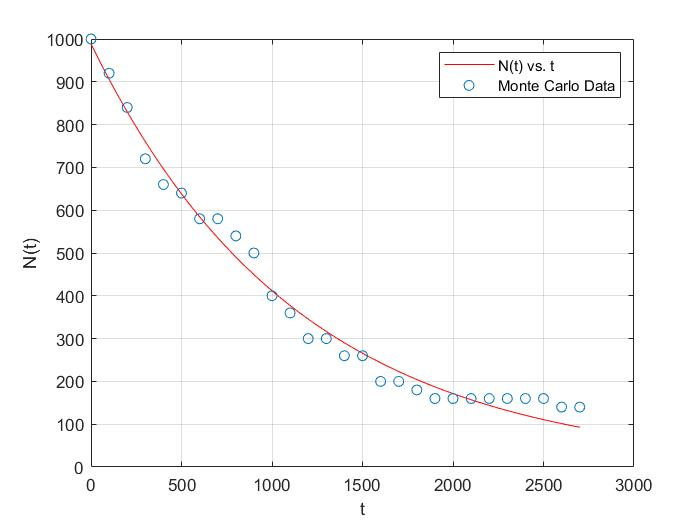
\includegraphics[width=7.5cm]{Q3/nrand_50} }}%
    \qquad
    \subfloat[\centering $Nrand=10^3$]{{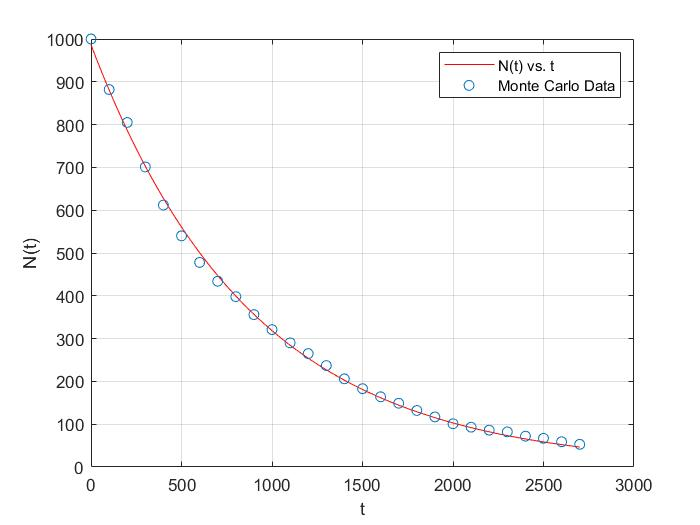
\includegraphics[width=7.5cm]{Q3/nrand_10e3} }}%
    \qquad
    \subfloat[\centering $Nrand=10^6$]{{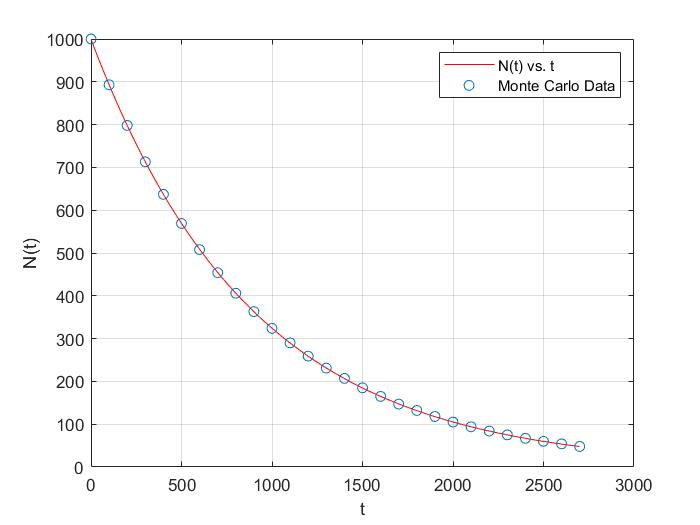
\includegraphics[width=7.5cm]{Q3/nrand_10e6} }}%
\  	\caption{Fit στα δεδομένα της μεθόδου για $Nrand=\{50,10^3,10^6\}$}
    \label{fig6}%
\end{figure}
	
%%%%%%%%%%%%%%%%%%%%%%%%%%%%%%%%%%%%%%%%%%%%%%%%%%     QUEST 4 %%%%%%%%%%%%%%%%%%%%%%%%%%%%%%%%%%%%%%%%%%%%
	\item[\textbf{Ερώτημα 4.}]	
	
	
		Τώρα τροποποιούμε τον κώδικα για τον υπολογισμό του π/4 ώστε να το υπολογίζει μέσω του ολοκληρώματος 
			\begin{align*}\label{eq5}
				\pi/4          =& \int_0^1 \frac{dx}{x^2+1}\Rightarrow\\
				\braket{\pi/4} =& \frac{1}{N}\sum\frac{1}{1+x^2} \numberthis
			\end{align*}
		Ο εν λόγω κώδικας υπάρχει τόσο στο αρχείο "pi2.m" όσο και παρακάτω 
		
		
	\begin{lstlisting}[language=Matlab]
		% find value of pi
%
Iseed1 = input('Enter random number seed: ');

Nrand = input('Enter number of random numbers to be generated: ');
%
rand('seed',Iseed1);
l1 = rand(1,Nrand);
n1 = 0;n2 = 0;f1 = 0 ;f2 = 0 ;
for k = 1:Nrand
   f1 = 1/((l1(k)).^2+1);
   f2 = f1*f1;
   n1 = n1 + f1;
   n2 = n2 + f2 ;
end
pi4   = n1/Nrand;
pi4_2 = n2/Nrand ;
erpi4 = sqrt((pi4_2-pi4.^2)/Nrand) ;
fprintf('<pi/4> = %f \n',pi4);
fprintf('delta<pi/4> = %f \n', erpi4);
	\end{lstlisting}
		
	Έτσι, επαναλαμβάνοντας τα βήματα του Ερωτήματος 2, δηλαδή τρέχοντας τον κώδικα για $seed=17$ και για $Nrand=\{10,10^2,10^3,10^4,10^5,10^6\}$ θα δούμε την συμπεριφορά της σύγκλισης του αλογρίθμου μέσω της γραφικής παράστασης $\braket{(\pi/4)} - Nrand$.
	
			\begin{table}[h!]
			\centering
			\begin{tabular}{r|r|r|r|r}
				$seed$ &  Nrand   & $\braket{\pi/4}$ & $\delta(\pi/4)$ \\ \hline \hline	
				17    &      $10^1$   &   0.747412   & 0.052303 \\
				17    &     $10^2$   &    0.783036   & 0.016838 \\
				17    &    $10^3$   &     0.789399   & 0.005132 \\
				17    &   $10^4$   &      0.784063   & 0.001620 \\
				17    &  $10^5$   &       0.785493   & 0.000508 \\	
				17    & $10^6$   &	      0.785319   & 0.000161 \\
				17    &$10^7$   &         0.785429   & 0.000051
		\end{tabular}
			\caption{Τιμές του π/4 για διάφορα πλήθη Nrand τυχαίων ζευγραριών με την μέθοδο του "p2.m"}
			\label{mat4}
		\end{table}
		
		
		
		Όσο αυξάνει το Nrand παρατηρούμε σύγκλιση στην πραγματική τιμή 0.785398 και όλοένα μειούμενο σφάλμα. Σε σύγκριση με την προηγούμενη μέθοδο του Ερωτήματος 2, αυτή ίσως είναι λίγο καλύτερη καθώς για $10^5$ αριθμούς έχουμε ήδη ακρίβεια στα 3 δεκαδικά ψηφία, ενώ με την πρώτη μέθοδο δεν είχαμε φτάσει καθόλου σε αυτή την ακρίβεια.
		Αυτό απεικονίζεται γραφικά και στην Εικόνα (\ref{fig7})
		
		\begin{figure}[h!]
			\centering
			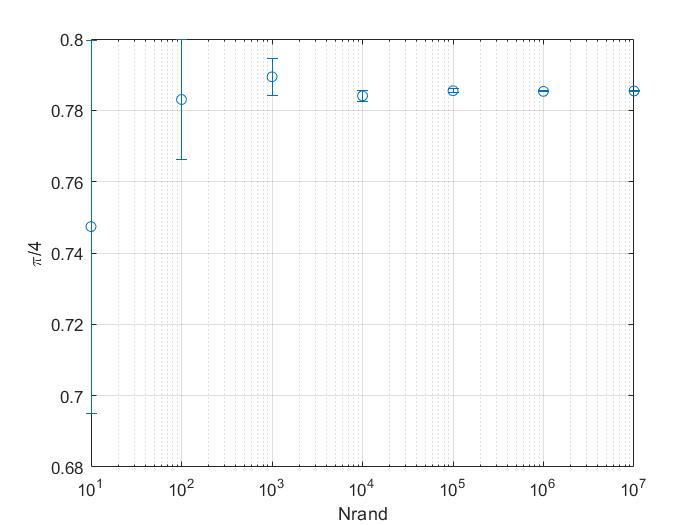
\includegraphics[scale=0.4]{Q4/nrand-pi4_correct.jpg}
			\caption{Γραφική παράσταση Nrand-$\braket{\pi/4}$ με την δεύτερη μέθοδο}
			\label{fig7}
		\end{figure}
		
		
		\newpage
%%%%%%%%%%%%%%%%%%%%%%%%%%%%%%%%%%%%%%%%     QUESTION 5      %%%%%%%%%%%%%%%%%%%%%%%%%%%%%%%%%%%%%%%%
	\item[\textbf{Ερώτημα 5.}]	
				
Ο τροποποιημένος κώδικας που περιέχει τον μετασχηματισμό $1+x_i^2$ φαίνεται παρακάτω και βρίσκεται επίσης στο αρχείο "example1\_mod.m". Στην ουσία έχει αλλαχθεί μόνο μία γραμμή, αυτή που σημειώνεται με **.


\begin{lstlisting}[language=Matlab]
% this is an example meant only for illustration
% uniformly distributed random numbers between 0 and 1
%
Iseed1 = input('Enter random number seed                       : ');
Nrand = input ('Enter number of random numbers to be generated : ');
Nbins = input ('Enter number of bins for the histo             : ');
%
rand('seed',Iseed1);
l1 = rand(1,Nrand);
%
if Nbins < 10
   Nbins = 10;
end
%
subplot(2,1,1),hist(l1,Nbins),title('distribution of random numbers'),... 
    xlabel('x_i '),...
subplot(2,1,2),hist((1-l1.^2),Nbins),xlabel( '1+x_i^2 ','interpreter','tex')%*************
%
    mo1 = mean(l1);
    sd1 = std(l1);
    var1 = var(l1);
    s12 = 0;
    s22 = 0;
    s23 = 0;
    for j=1:Nbins
        athr1(j) = 0;
    end
    for k=1:Nrand
        s12 = s12 + (((l1(k))-mo1)^2) ;
        ibin1 = (round(l1(k) * Nbins)) ;
        ibin2 = (round((l1(k)+(0.5/Nbins)) * Nbins)) ;
        if ibin1 >= ibin2;
            ibin = ibin1;
        else
            ibin = ibin2;
        end
        athr1(ibin) = athr1(ibin) + 1;
    end
    s1 = s12/(Nrand -1) ;
subplot; 
for j=1:Nbins
    s22 = s22 + athr1(j);
end
s2 = s22/Nbins;
for j=1:Nbins
    s23 = s23 + (((athr1(j))-s2)^2) ;
end
s3 = sqrt(s23)/(Nbins -1) ;
vary = std(athr1);
sigy = s3;
sigpery = s3/s2;
fprintf('meany = %f \n', s2);
fprintf('sigy = %f \n', s3);
fprintf('percent = %f \n', sigpery);

	\end{lstlisting}				

Τώρα παίρνουμε seed=17, $Nrand=10^5$ και $bins=\{10,100\}$ και τα αποτελέσματα φαίνονται στην παρακάτω Εικόνα (\ref{fig8}a-b).

\begin{figure}[h!]
    \centering
    \subfloat[\centering bins=10]{{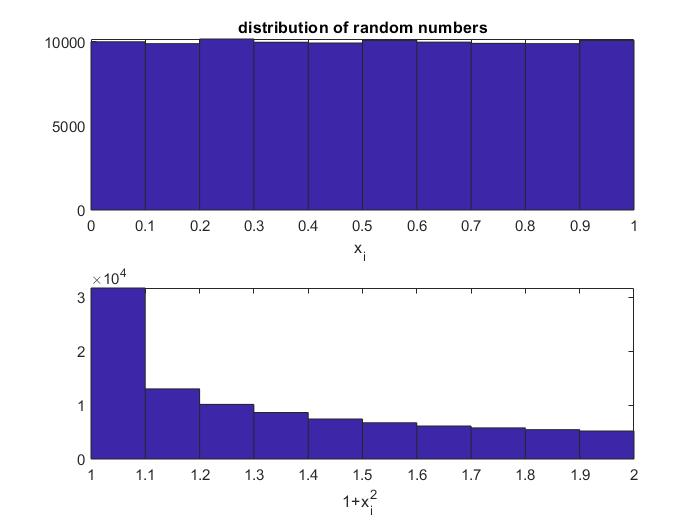
\includegraphics[width=7cm]{Q5/bins_10} }}%
    \qquad
    \subfloat[\centering bins=100]{{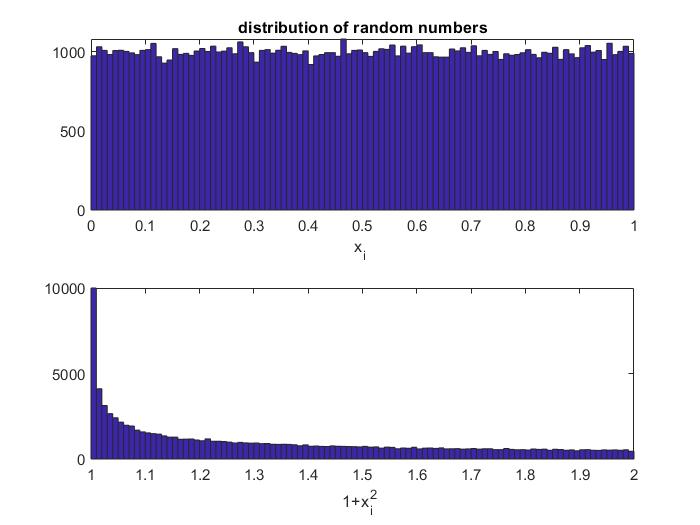
\includegraphics[width=7cm]{Q5/bins_100.jpg} }}%
    
    \caption{Nrand=$10^5$ για την $1+x^2$}%
    \label{fig8}%
\end{figure}

	Και στις δύο περιπτώσεις επειδή έχουμε πάρει $0<x_i<1$ ισχύει ότι $0<x_i^2<1\Rightarrow 0<x_1^2+1<1$. Παρατηρούμε ότι οι περισσότεροι αριθμοί συγκεντώνονται κοντά στο 1. Έχουμε ότι $sqrt(0.1)\simeq0.31$. Αυτό σημαίνει πως περίπου το 30\% των συνολικών αριθμών, δηλαδή περίπου $0.3\cdot10^5=0.3\cdot10^4$, είναι συγκεντρωμένοι μεταξύ 1 και 1.1. Αυτό είναι πιό εμφανές στην Εικόνα (\ref{fig8}a) όπου έχουμε λιγότερα bins και βλέπουμε πως όντως περίπου $3\times10^4$ αριθμοί βρίσκονται εως το 1.1. Καθώς αυξάνονται τα bins οι αριθμοί μαζεύκονται όλο και πιό κοντά στο 1.

%%%%%%%%%%%%%%%%%%%%%%%%%%%%%%%%%%%%%%%%     QUESTION 6      %%%%%%%%%%%%%%%%%%%%%%%%%%%%%%%%%%%%%%%%		
	\item[\textbf{Ερώτημα 6.}]	
	Εδώ θα υπολογίσουμε πάλι το π/4 με μία άλλη μέθοδο που μοιάζει με εκείνη του Ερωτήματος 4 αλλά περιλαμβάνει μία συνάρτηση βάρους w(x) η οποία βελτιώνει την σύγκλιση. Δηλαδή θέλουμε να υπολογίσουμε ένα ολοκλήρωμα της μορφής 
		\begin{align*}\label{eq6}
			I = \int_{x_-}^{x_+} f(x)dx = \int_{x_-}^{x_+} w(x) \frac{f(x)}{w(x)}dx \numberthis
		\end{align*}
	
	Η συνάρτηση βάρους πρέπει να έχει κάποιες ιδιότητες όπως να είναι θετική, να είναι κανονικοποιημένη στην μονάδα και χρησιμοποιείται όταν η αρχική f(x) παίνει μεγάλες τιμές για ένα μικρό διάστημα του πεδίου ορισμού της γύρω από ένα $x_0$ και πανού αλλού είναι 0. Τότε, οι τυχαίοι αριθμοί που προέρχονται π.χ. από μία ομοιόμορφη κατανομή θα έχουν ίδια πιθανότητα να είναι σε όλο το διάστημα ενδιαφέροντός μας, άρα οι περισσότεροι θα βρίσκονται εκτός της κορυφής, με αποτέλεσμα τον αναποτελεσματικό υπολογισμό του Ι. Γι' αυτό χρησιμοποιούμε την συνάρτηση βάρους w(x) η οποία εξομαλύνει την αρχική f(x). 
	
	Εμείς θα χρησιμοποιήσουμε την 
		\begin{equation}\label{eq7}
			w(x) = \frac{4-2x}{3}			
		\end{equation}
	
	Τώρα στο ολοκλήρωμα (\ref{eq6}) κάνουμε την παρακάτω αλλαγή μεταβλητών 
		\begin{align*}\label{eq8}
			\odv{y}{x} =& w(x)  \numberthis\\ 
			y(x_-) =& 0 \\ 
			y(x_+) =& 1
		\end{align*}
		
Άρα από τις (\ref{eq6})\&(\ref{eq8}) έχουμε 
	\begin{align*}\label{eq9}
		I     =& \int_{y(x_-)}^{y(x_+)} \frac{f(x(y))}{w(x(y))} w(x)dx \Rightarrow\\
		      =& \int_0^1   \frac{f(x(y))}{w(x(y))} dy\Rightarrow  \numberthis\\
		I\simeq& \frac{1}{N} \sum_i\frac{f(x(y_i))}{w(x(y_i))} \pm \sqrt{\frac{(\braket{f/w})^2 - \braket{f/w}^2}{N}} \numberthis
	\end{align*}			
		
	Απομένει δηλαδή να βρούμε την συνάρτηση x(y).	Από την σχέση (\ref{eq8}) έχουμε 	
		\begin{align*}
			\odv{y}{x} =& w(x) \Rightarrow\\
			y(x)       =& \int w(x) dx  = \int \frac{4-2x}{3}dx\Rightarrow\\
			y(x)       =& \frac{x(4-x)}{3} \Rightarrow \\ 
			x^2        -&  4x +3y = 0 \Rightarrow
		\end{align*}
		\begin{equation}\label{eq11}
    \left\{
    \begin{matrix}
    	x_1 =& 2+\sqrt{4-3y}\Rightarrow x_1(0) = 4, x_1(1) = 3 \text{ , άρα απορρίπτεται} \\ 
    	x_2 =& 2-\sqrt{4-3y}\Rightarrow x_2(0) = 0, x_2(1) = 1 \text{ , άρα το κρατάμε}
    \end{matrix}
    \right.
		\end{equation}
		
Άρα η προσέγγιση του ολοκληρώματος (\ref{eq9}) από την σχέση (10) γίνεται 
	\begin{align*}\label{eq12}
			I\simeq& \frac{1}{N} \sum_{i=1}^N\frac{f(2-\sqrt{4-3y_i})}{w(2-\sqrt{4-3y_i})} \pm \sqrt{\frac{\braket{(f/w)^2} - \braket{f/w}^2}{N}}    \numberthis
	\end{align*}			
Αν η υπο ολοκλήρωση συνάρτηση είναι η $f(x) = 1/(x^2+1)$ και η συνάρτηση βάρους η $w(x)= (4-2x)/3$ τότε ο λόγος τους συναρτήσει του y είναι 
	\begin{align*}\label{eq13}
		\phi(y) =& \frac{f(x(y))}{w(x(y))}  = \frac{f(2-\sqrt{4-3y})}{w(2-\sqrt{4-3y}) \numberthis}% \Rightarrow\\
		        %=& \frac{1}{1+ (2-\sqrt{4-3y})^2} \frac{3}{4-2(2-\sqrt{4-3y})}          \Rightarrow\\ 
		        %=& \frac{1}{1+ (2-\sqrt{4-3y})^2} \frac{3}{2\sqrt{4-3y}}
	\end{align*}
		
	Έτσι αλλάζουμε τον κώδικα του "pi2.m" ώστε να υπολογίζει το ολοκλήρωμα της $\phi(y)$. Ο κώδικας φάινεται παρακάτω καθώς και στο αρχείο "pi3.m"
		
	\begin{lstlisting}[language=Matlab]
	% find value of pi
Iseed1 = input('Enter random number seed                     : ');
Nrand = input('Enter number of random numbers to be generated: ');

rand('seed',Iseed1);
l1 = rand(1,Nrand);

n1 = 0;n2 = 0;f1 = 0 ;f2 = 0 ;
for k = 1:Nrand
%    f1 = 1/((l1(k)).^2+1);
%    f2 = f1*f1;
%    n1 = n1 + f1;
%    n2 = n2 + f2 ;
   
   xofy  = 2 - sqrt(4-3*l1(k));
   f     = 1/(1+xofy^2)      ; 
   w     = (4 - 2*xofy)/3      ;
   f1    = f./w               ;
   f2    = f1*f1              ; 
   n1    = n1+f1; 
   n2    = n2+f2;  
   
end
pi4   = n1/Nrand;
pi4_2 = n2/Nrand ;
erpi4 = sqrt((pi4_2-pi4.^2)/Nrand) ;

%erpi4 = (1/Nrand)*(sqrt((coun1*(Nrand-coun1)/Nrand)));
fprintf('<pi/4> = %f \n',pi4);
fprintf('delta<pi/4> = %f \n', erpi4);

%fprintf('|pi/4 - pi/4_estimated |= %f\n', abs(pi/4-pi4))
	\end{lstlisting}		
		
		
Τρέχουμε το πρόγραμμα "pi4.m" για διάφορες τιμές του $Nrand=\{10,10^2,10^3,10^4,10^5,10^6,10^7\}$. Τα αποτελέσματα φαίνονται στον Πίνακα (\ref{mat5}). Επίσης, στην Εικόνα (\ref{fig9}) φαίνεται η γραφική παράσταση Nrand-$\braket{\pi/4}$.
		\begin{table}[h!]
			\centering
			\begin{tabular}{r|r|r|r|r}
				$seed$ &  Nrand   & $\braket{\pi/4}$ & $\delta(\pi/4)$ \\ \hline \hline	
				17    &      $10^1$   &   0.783348   & 0.007015 \\
				17    &     $10^2$   &    0.783014   & 0.001976 \\
				17    &    $10^3$   &     0.785463   & 0.000639 \\
				17    &   $10^4$   &      0.785109   & 0.000201 \\
				17    &  $10^5$   &       0.785416   & 0.000063 \\	
				17    & $10^6$   &	      0.785376   & 0.000020 \\
				17    &$10^7$   &         0.785395   & 0.000006
		\end{tabular}
			\caption{Τιμές του π/4=0.785398 για διάφορα πλήθη Nrand τυχαίων ζευγραριών με την μέθοδο του "p3.m"}
			\label{mat5}
		\end{table}
			%\vspace{-1cm}
		\begin{figure}[h!]
		\centering 
			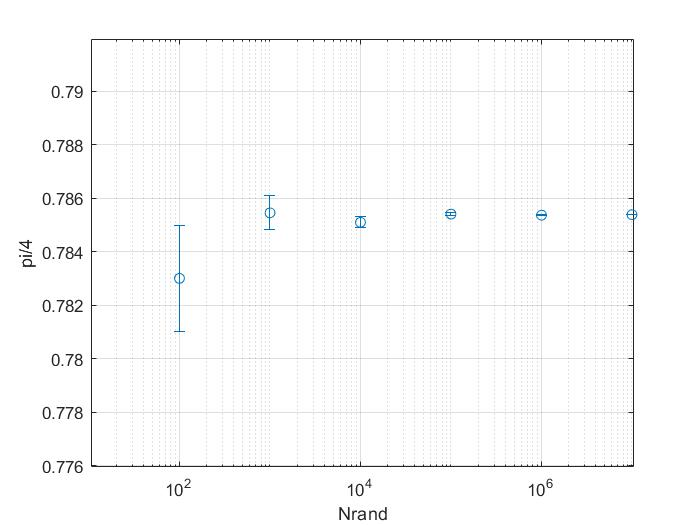
\includegraphics[scale=0.4]{Q6/nrand-pi4}	
			\caption{Γραφική Παράσταση Nrand-$\braket{\pi/4}$ με την τρίτη μέθοδο}		
			\label{fig9}
		\end{figure}
		

		Τώρα θα προχωρήσουμε σε μία στοιχειώδη σύγκριση των τριών παραπάνω μεθόδων. Αρχικά, παρατηρούμε αμέσως πως η τρίτη έχει δώσει τον π/4 με την μεγαλύτερη ακρίβεια από όλες. Ακόμη, όπως βλέπουμε στην Εικόνα (\ref{fig10}) η πρώτη μέθοδος είναι η χειρότερη τόσο από ακρίβεια όσο και από πλευράς ταχύτητας σύγκλισης που πλησιάζει το π/4. 
		Ακόμη, από την Εικόνα (\ref{fig11}) φάινεται ότι οι μέθοδοι 2,3 έχουν ίδια ταχύτητα σύγκλισης και ακρίβεια, ωστόσο από τους αντίστοιχους Πίνακες (\ref{mat4}) \& (\ref{mat5}) βλέπουμε πως η μέθοδος 3 είναι πιό αποτελεσματική καθώς δίνει το π/4 με μεγαλύτερη ακρίβεια.
		
		\begin{figure}[h!] 
			\centering 
			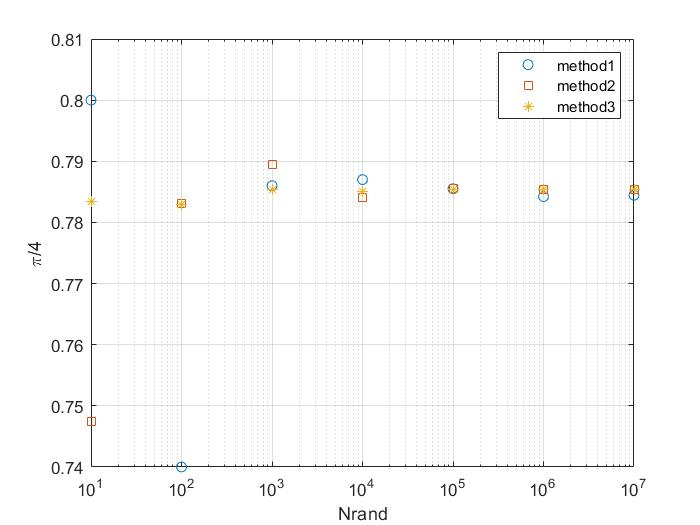
\includegraphics[scale=0.45]{Q6/compare_1}
			\caption{Φαίνονται οι γραφικές $\braket{\pi/4}-Nrand$ για τις τρεις μεθόδους.}
			\label{fig10}
		\end{figure}
		
		
		\begin{figure}[h!] 
			\centering 
			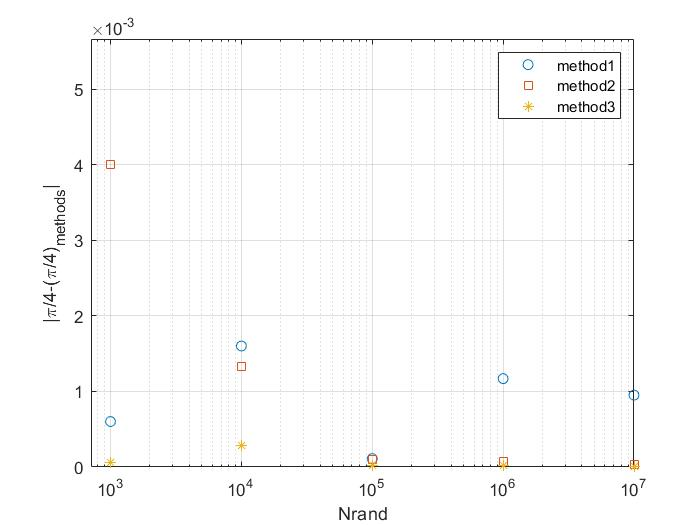
\includegraphics[scale=0.5]{Q6/compare_2}
			\caption{Φαίνονται οι γραφικές $|\braket{\pi/4}-\pi/4|-Nrand$ για τις τρεις μεθόδους για μεγάλα Ntrans.}
			\label{fig11}
		\end{figure}
			
		
\end{enumerate}



\end{document}